\documentclass[border=10pt]{standalone}

\usepackage{tikz}
\usepackage{tikzsymbols}
\usetikzlibrary{calc,patterns,shapes.geometric}

\def\centerarc[#1](#2)(#3:#4:#5){\draw[#1] ($(#2)+({#5*cos(#3)},{#5*sin(#3)})$) arc (#3:#4:#5);}

\begin{document}
	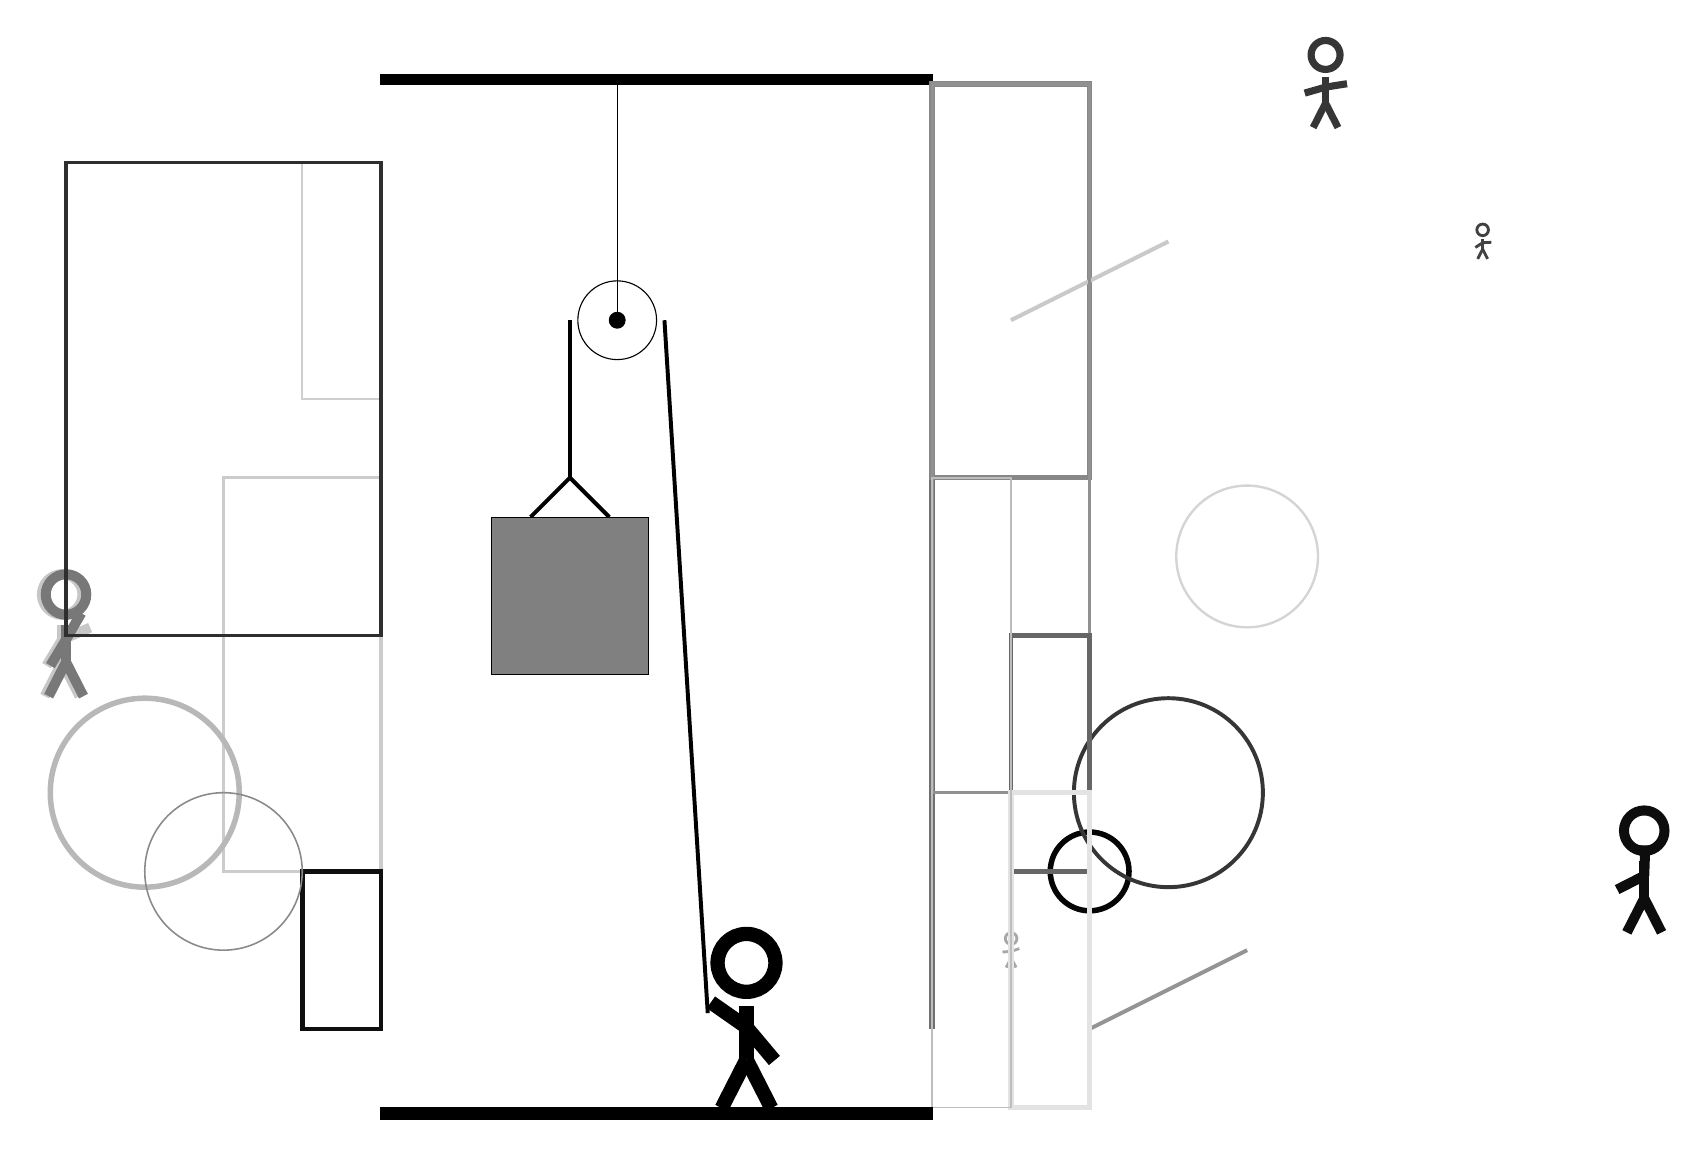
\begin{tikzpicture}
		%%%%% START %%%%%
		
		\draw[fill=black] (-2, 10) rectangle (5, 10.125);
		
		\draw (1, 7) circle (0.5);
		\draw[fill=black] (1, 7) circle (0.1);
		\draw (1, 10) -- (1, 7);
		
		\draw [line width=0.7mm, color=black!98](7, 0) circle (0.5);
		
		\draw[line width=0.4mm, color=black!20] (-4, 5) rectangle (-2, 0);
		\node[line width=0.4mm, color=black!22] at (-6, 3) {\Strichmaxerl[7][59][23]};
		\node[line width=0.2mm, color=black!74] at (12, 8) {\Strichmaxerl[2][33][3]};
		\draw[line width=0.6mm, color=black!94] (-3, 0) rectangle (-2, -2);
		\node[line width=0.6mm, color=black!53] at (-6, 3) {\Strichmaxerl[7][59][60]};
		\draw [line width=0.7mm, color=black!28](-5, 1) circle (1.2);
		
		\draw[line width=0.2mm, color=black!19] (-3, 6) rectangle (-2, 9);
		\draw [line width=0.6mm, color=black!99](10, 9) circle (0.0);
		
		\draw[line width=0.5mm, color=black!42](9, -1) -- (7, -2);
		\draw [line width=0.4mm, color=black!82](-4, 8) circle (0.0);
		\draw [line width=0.2mm, color=black!46](-4, 0) circle (1.0);
		\draw [line width=0.5mm, color=black!79](8, 1) circle (1.2);
		
		\draw[line width=0.7mm, color=black!56] (5, 7) rectangle (5, -2);
		\draw[line width=0.7mm, color=black!47] (7, 5) rectangle (5, 10);
		\draw[line width=0.5mm, color=black!21](8, 8) -- (6, 7);
		
		\draw[line width=0.4mm, color=black!82] (-2, 9) rectangle (-6, 3);
		\draw[line width=0.4mm, color=black!43] (5, 10) rectangle (7, 1);
		\draw[line width=0.6mm, color=black!60] (6, 3) rectangle (7, 0);
		\node[line width=0.7mm, color=black!34] at (6, -1) {\Strichmaxerl[2][4][19]};
		\draw[line width=0.7mm, color=black!11] (7, 1) rectangle (6, -3);
		
		\node[line width=0.7mm, color=black!95] at (14, 0) {\Strichmaxerl[7][27][88]};
		\draw [line width=0.2mm, color=black!15](-3, 7) circle (0.0);
		\draw [line width=0.3mm, color=black!17](9, 4) circle (0.9);
		\draw[line width=0.2mm, color=black!26] (5, -3) rectangle (6, 5);
		
		\node[line width=0.5mm, color=black!79] at (10, 10) {\Strichmaxerl[5][16][9]};
		
		\draw[line width=0.5mm] (-0.1, 4.5) -- (0.4, 5.0) -- (0.9, 4.5);
		\draw[fill=black!50] (-0.6, 4.5) rectangle (1.4, 2.5);
		
		\draw[line width=0.5mm] (0.4, 7) -- (0.4, 5.0);
		\centerarc[line width=0.5mm](1, 7)(0:180:0.6);
		\draw[line width=0.5mm](1.6, 7) -- (2.15, -1.8);
		
		\node at (2.6, -1.9) {\Strichmaxerl[10][-35][-50]};
		
		\draw[fill=black] (-2, -3) rectangle (5, -3.15);
		
		%%%%% END %%%%%
	\end{tikzpicture}
\end{document}